
%% bare_jrnl.tex
%% V1.4b
%% 2015/08/26
%% by Michael Shell
%% see http://www.michaelshell.org/
%% for current contact information.
%%
%% This is a skeleton file demonstrating the use of IEEEtran.cls
%% (requires IEEEtran.cls version 1.8b or later) with an IEEE
%% journal paper.
%%
%% Support sites:
%% http://www.michaelshell.org/tex/ieeetran/
%% http://www.ctan.org/pkg/ieeetran
%% and
%% http://www.ieee.org/

%%*************************************************************************
%% Legal Notice:
%% This code is offered as-is without any warranty either expressed or
%% implied; without even the implied warranty of MERCHANTABILITY or
%% FITNESS FOR A PARTICULAR PURPOSE! 
%% User assumes all risk.
%% In no event shall the IEEE or any contributor to this code be liable for
%% any damages or losses, including, but not limited to, incidental,
%% consequential, or any other damages, resulting from the use or misuse
%% of any information contained here.
%%
%% All comments are the opinions of their respective authors and are not
%% necessarily endorsed by the IEEE.
%%
%% This work is distributed under the LaTeX Project Public License (LPPL)
%% ( http://www.latex-project.org/ ) version 1.3, and may be freely used,
%% distributed and modified. A copy of the LPPL, version 1.3, is included
%% in the base LaTeX documentation of all distributions of LaTeX released
%% 2003/12/01 or later.
%% Retain all contribution notices and credits.
%% ** Modified files should be clearly indicated as such, including  **
%% ** renaming them and changing author support contact information. **
%%*************************************************************************


% *** Authors should verify (and, if needed, correct) their LaTeX system  ***
% *** with the testflow diagnostic prior to trusting their LaTeX platform ***
% *** with production work. The IEEE's font choices and paper sizes can   ***
% *** trigger bugs that do not appear when using other class files.       ***                          ***
% The testflow support page is at:
% http://www.michaelshell.org/tex/testflow/



%\documentclass[journal]{./sty/IEEEtran}
%
% If IEEEtran.cls has not been installed into the LaTeX system files,
% manually specify the path to it like:
% \documentclass[journal]{../sty/IEEEtran}





% Some very useful LaTeX packages include:
% (uncomment the ones you want to load)


% *** MISC UTILITY PACKAGES ***
%
%\usepackage{ifpdf}
% Heiko Oberdiek's ifpdf.sty is very useful if you need conditional
% compilation based on whether the output is pdf or dvi.
% usage:
% \ifpdf
%   % pdf code
% \else
%   % dvi code
% \fi
% The latest version of ifpdf.sty can be obtained from:
% http://www.ctan.org/pkg/ifpdf
% Also, note that IEEEtran.cls V1.7 and later provides a builtin
% \ifCLASSINFOpdf conditional that works the same way.
% When switching from latex to pdflatex and vice-versa, the compiler may
% have to be run twice to clear warning/error messages.






% *** CITATION PACKAGES ***
%
%\usepackage{cite}
% cite.sty was written by Donald Arseneau
% V1.6 and later of IEEEtran pre-defines the format of the cite.sty package
% \cite{} output to follow that of the IEEE. Loading the cite package will
% result in citation numbers being automatically sorted and properly
% "compressed/ranged". e.g., [1], [9], [2], [7], [5], [6] without using
% cite.sty will become [1], [2], [5]--[7], [9] using cite.sty. cite.sty's
% \cite will automatically add leading space, if needed. Use cite.sty's
% noadjust option (cite.sty V3.8 and later) if you want to turn this off
% such as if a citation ever needs to be enclosed in parenthesis.
% cite.sty is already installed on most LaTeX systems. Be sure and use
% version 5.0 (2009-03-20) and later if using hyperref.sty.
% The latest version can be obtained at:
% http://www.ctan.org/pkg/cite
% The documentation is contained in the cite.sty file itself.






% *** GRAPHICS RELATED PACKAGES ***
%
%\ifCLASSINFOpdf
  % \usepackage[pdftex]{graphicx}
  % declare the path(s) where your graphic files are
  % \graphicspath{{../pdf/}{../jpeg/}}
  % and their extensions so you won't have to specify these with
  % every instance of \includegraphics
  % \DeclareGraphicsExtensions{.pdf,.jpeg,.png}
%\else
  % or other class option (dvipsone, dvipdf, if not using dvips). graphicx
  % will default to the driver specified in the system graphics.cfg if no
  % driver is specified.
  % \usepackage[dvips]{graphicx}
  % declare the path(s) where your graphic files are
  % \graphicspath{{../eps/}}
  % and their extensions so you won't have to specify these with
  % every instance of \includegraphics
  % \DeclareGraphicsExtensions{.eps}
%\fi
% graphicx was written by David Carlisle and Sebastian Rahtz. It is
% required if you want graphics, photos, etc. graphicx.sty is already
% installed on most LaTeX systems. The latest version and documentation
% can be obtained at: 
% http://www.ctan.org/pkg/graphicx
% Another good source of documentation is "Using Imported Graphics in
% LaTeX2e" by Keith Reckdahl which can be found at:
% http://www.ctan.org/pkg/epslatex
%
% latex, and pdflatex in dvi mode, support graphics in encapsulated
% postscript (.eps) format. pdflatex in pdf mode supports graphics
% in .pdf, .jpeg, .png and .mps (metapost) formats. Users should ensure
% that all non-photo figures use a vector format (.eps, .pdf, .mps) and
% not a bitmapped formats (.jpeg, .png). The IEEE frowns on bitmapped formats
% which can result in "jaggedy"/blurry rendering of lines and letters as
% well as large increases in file sizes.
%
% You can find documentation about the pdfTeX application at:
% http://www.tug.org/applications/pdftex





% *** MATH PACKAGES ***
%
%\usepackage{amsmath}
% A popular package from the American Mathematical Society that provides
% many useful and powerful commands for dealing with mathematics.
%
% Note that the amsmath package sets \interdisplaylinepenalty to 10000
% thus preventing page breaks from occurring within multiline equations. Use:
%\interdisplaylinepenalty=2500
% after loading amsmath to restore such page breaks as IEEEtran.cls normally
% does. amsmath.sty is already installed on most LaTeX systems. The latest
% version and documentation can be obtained at:
% http://www.ctan.org/pkg/amsmath





% *** SPECIALIZED LIST PACKAGES ***
%
%\usepackage{algorithmic}
% algorithmic.sty was written by Peter Williams and Rogerio Brito.
% This package provides an algorithmic environment fo describing algorithms.
% You can use the algorithmic environment in-text or within a figure
% environment to provide for a floating algorithm. Do NOT use the algorithm
% floating environment provided by algorithm.sty (by the same authors) or
% algorithm2e.sty (by Christophe Fiorio) as the IEEE does not use dedicated
% algorithm float types and packages that provide these will not provide
% correct IEEE style captions. The latest version and documentation of
% algorithmic.sty can be obtained at:
% http://www.ctan.org/pkg/algorithms
% Also of interest may be the (relatively newer and more customizable)
% algorithmicx.sty package by Szasz Janos:
% http://www.ctan.org/pkg/algorithmicx




% *** ALIGNMENT PACKAGES ***
%
%\usepackage{array}
% Frank Mittelbach's and David Carlisle's array.sty patches and improves
% the standard LaTeX2e array and tabular environments to provide better
% appearance and additional user controls. As the default LaTeX2e table
% generation code is lacking to the point of almost being broken with
% respect to the quality of the end results, all users are strongly
% advised to use an enhanced (at the very least that provided by array.sty)
% set of table tools. array.sty is already installed on most systems. The
% latest version and documentation can be obtained at:
% http://www.ctan.org/pkg/array


% IEEEtran contains the IEEEeqnarray family of commands that can be used to
% generate multiline equations as well as matrices, tables, etc., of high
% quality.




% *** SUBFIGURE PACKAGES ***
%\ifCLASSOPTIONcompsoc
%  \usepackage[caption=false,font=normalsize,labelfont=sf,textfont=sf]{subfig}
%\else
%\usepackage[caption=false,font=footnotesize]{./sty/subfig}
%\fi
% subfig.sty, written by Steven Douglas Cochran, is the modern replacement
% for subfigure.sty, the latter of which is no longer maintained and is
% incompatible with some LaTeX packages including fixltx2e. However,
% subfig.sty requires and automatically loads Axel Sommerfeldt's caption.sty
% which will override IEEEtran.cls' handling of captions and this will result
% in non-IEEE style figure/table captions. To prevent this problem, be sure
% and invoke subfig.sty's "caption=false" package option (available since
% subfig.sty version 1.3, 2005/06/28) as this is will preserve IEEEtran.cls
% handling of captions.
% Note that the Computer Society format requires a larger sans serif font
% than the serif footnote size font used in traditional IEEE formatting
% and thus the need to invoke different subfig.sty package options depending
% on whether compsoc mode has been enabled.
%
% The latest version and documentation of subfig.sty can be obtained at:
% http://www.ctan.org/pkg/subfig




% *** FLOAT PACKAGES ***
%
%\usepackage{fixltx2e}
% fixltx2e, the successor to the earlier fix2col.sty, was written by
% Frank Mittelbach and David Carlisle. This package corrects a few problems
% in the LaTeX2e kernel, the most notable of which is that in current
% LaTeX2e releases, the ordering of single and double column floats is not
% guaranteed to be preserved. Thus, an unpatched LaTeX2e can allow a
% single column figure to be placed prior to an earlier double column
% figure.
% Be aware that LaTeX2e kernels dated 2015 and later have fixltx2e.sty's
% corrections already built into the system in which case a warning will
% be issued if an attempt is made to load fixltx2e.sty as it is no longer
% needed.
% The latest version and documentation can be found at:
% http://www.ctan.org/pkg/fixltx2e


%\usepackage{stfloats}
% stfloats.sty was written by Sigitas Tolusis. This package gives LaTeX2e
% the ability to do double column floats at the bottom of the page as well
% as the top. (e.g., "\begin{figure*}[!b]" is not normally possible in
% LaTeX2e). It also provides a command:
%\fnbelowfloat
% to enable the placement of footnotes below bottom floats (the standard
% LaTeX2e kernel puts them above bottom floats). This is an invasive package
% which rewrites many portions of the LaTeX2e float routines. It may not work
% with other packages that modify the LaTeX2e float routines. The latest
% version and documentation can be obtained at:
% http://www.ctan.org/pkg/stfloats
% Do not use the stfloats baselinefloat ability as the IEEE does not allow
% \baselineskip to stretch. Authors submitting work to the IEEE should note
% that the IEEE rarely uses double column equations and that authors should try
% to avoid such use. Do not be tempted to use the cuted.sty or midfloat.sty
% packages (also by Sigitas Tolusis) as the IEEE does not format its papers in
% such ways.
% Do not attempt to use stfloats with fixltx2e as they are incompatible.
% Instead, use Morten Hogholm'a dblfloatfix which combines the features
% of both fixltx2e and stfloats:
%
% \usepackage{dblfloatfix}
% The latest version can be found at:
% http://www.ctan.org/pkg/dblfloatfix




%\ifCLASSOPTIONcaptionsoff
%  \usepackage[nomarkers]{endfloat}
% \let\MYoriglatexcaption\caption
% \renewcommand{\caption}[2][\relax]{\MYoriglatexcaption[#2]{#2}}
%\fi
% endfloat.sty was written by James Darrell McCauley, Jeff Goldberg and 
% Axel Sommerfeldt. This package may be useful when used in conjunction with 
% IEEEtran.cls'  captionsoff option. Some IEEE journals/societies require that
% submissions have lists of figures/tables at the end of the paper and that
% figures/tables without any captions are placed on a page by themselves at
% the end of the document. If needed, the draftcls IEEEtran class option or
% \CLASSINPUTbaselinestretch interface can be used to increase the line
% spacing as well. Be sure and use the nomarkers option of endfloat to
% prevent endfloat from "marking" where the figures would have been placed
% in the text. The two hack lines of code above are a slight modification of
% that suggested by in the endfloat docs (section 8.4.1) to ensure that
% the full captions always appear in the list of figures/tables - even if
% the user used the short optional argument of \caption[]{}.
% IEEE papers do not typically make use of \caption[]'s optional argument,
% so this should not be an issue. A similar trick can be used to disable
% captions of packages such as subfig.sty that lack options to turn off
% the subcaptions:
% For subfig.sty:
% \let\MYorigsubfloat\subfloat
% \renewcommand{\subfloat}[2][\relax]{\MYorigsubfloat[]{#2}}
% However, the above trick will not work if both optional arguments of
% the \subfloat command are used. Furthermore, there needs to be a
% description of each subfigure *somewhere* and endfloat does not add
% subfigure captions to its list of figures. Thus, the best approach is to
% avoid the use of subfigure captions (many IEEE journals avoid them anyway)
% and instead reference/explain all the subfigures within the main caption.
% The latest version of endfloat.sty and its documentation can obtained at:
% http://www.ctan.org/pkg/endfloat
%
% The IEEEtran \ifCLASSOPTIONcaptionsoff conditional can also be used
% later in the document, say, to conditionally put the References on a 
% page by themselves.




% *** PDF, URL AND HYPERLINK PACKAGES ***
%
%\usepackage{url}
% url.sty was written by Donald Arseneau. It provides better support for
% handling and breaking URLs. url.sty is already installed on most LaTeX
% systems. The latest version and documentation can be obtained at:
% http://www.ctan.org/pkg/url
% Basically, \url{my_url_here}.




% *** Do not adjust lengths that control margins, column widths, etc. ***
% *** Do not use packages that alter fonts (such as pslatex).         ***
% There should be no need to do such things with IEEEtran.cls V1.6 and later.
% (Unless specifically asked to do so by the journal or conference you plan
% to submit to, of course. )


%% DOCUMENT CLASS %%%%%%%%%
\documentclass[journal]{./sty/IEEEtran}





%% USER USED PACKAGES %%%%%%%
\usepackage{fixltx2e}
\usepackage{amsmath}
\usepackage{amsfonts}
\usepackage{cite}
\usepackage{array}
\usepackage{booktabs}
\usepackage{mathtools}
\usepackage{tabularx}
\usepackage{graphicx}
\usepackage{subfig}
\graphicspath{ {./images/} }
\usepackage[caption=false,font=footnotesize]{./sty/subfig}


\newcommand{\hquad}{\hspace{0.5em}}
\begin{document}
%
% paper title
% Titles are generally capitalized except for words such as a, an, and, as,
% at, but, by, for, in, nor, of, on, or, the, to and up, which are usually
% not capitalized unless they are the first or last word of the title.
% Linebreaks \\ can be used within to get better formatting as desired.
% Do not put math or special symbols in the title.
\title{On the synthesis and design of a novel backdrivable high-stiffness capstan drive}
%
%
% author names and IEEE memberships
% note positions of commas and nonbreaking spaces ( ~ ) LaTeX will not break
% a structure at a ~ so this keeps an author's name from being broken across
% two lines.
% use \thanks{} to gain access to the first footnote area
% a separate \thanks must be used for each paragraph as LaTeX2e's \thanks
% was not built to handle multiple paragraphs
%

\author{Jordan M. Longval~%\IEEEmembership{Member,~IEEE,}
       and Clément Gosselin~
        %and~Jane~Doe,~%\IEEEmembership{Life~Fellow,~IEEE}% <-this % stops a space
\thanks{J. Longval and C. Gosselin are with  the Department of Mechanical Engineering, Université Laval, Québec, Canada e-mail:gosselin@gmc.ulaval.ca.}}
%\thanks{Manuscript received April 19, 2005; revised August 26, 2015.}}

% note the % following the last \IEEEmembership and also \thanks - 
% these prevent an unwanted space from occurring between the last author name
% and the end of the author line. i.e., if you had this:
% 
% \author{....lastname \thanks{...} \thanks{...} }
%                     ^------------^------------^----Do not want these spaces!
%
% a space would be appended to the last name and could cause every name on that
% line to be shifted left slightly. This is one of those "LaTeX things". For
% instance, "\textbf{A} \textbf{B}" will typeset as "A B" not "AB". To get
% "AB" then you have to do: "\textbf{A}\textbf{B}"
% \thanks is no different in this regard, so shield the last } of each \thanks
% that ends a line with a % and do not let a space in before the next \thanks.
% Spaces after \IEEEmembership other than the last one are OK (and needed) as
% you are supposed to have spaces between the names. For what it is worth,
% this is a minor point as most people would not even notice if the said evil
% space somehow managed to creep in.



% The paper headers
\markboth{IEEE Robotics and Automation Letters}%
{Shell \MakeLowercase{\textit{et al.}}: Bare Demo of IEEEtran.cls for IEEE Journals}
% The only time the second header will appear is for the odd numbered pages
% after the title page when using the twoside option.
% 
% *** Note that you probably will NOT want to include the author's ***
% *** name in the headers of peer review papers.                   ***
% You can use \ifCLASSOPTIONpeerreview for conditional compilation here if
% you desire.




% If you want to put a publisher's ID mark on the page you can do it like
% this:
%\IEEEpubid{0000--0000/00\$00.00~\copyright~2015 IEEE}
% Remember, if you use this you must call \IEEEpubidadjcol in the second
% column for its text to clear the IEEEpubid mark.



% use for special paper notices
%\IEEEspecialpapernotice{(Invited Paper)}




% make the title area
\maketitle

% As a general rule, do not put math, special symbols or citations
% in the abstract or keywords.
\begin{abstract}
This article introduces a novel backdrivable high-stiffness cable capstan drive architecture for robotics applications. The drive has a low transmission ratio and a higher stiffness than typical capstan drives. The higher transmission stiffness is obtained by the use of grooves on both the input and the output pulleys of the drive which increases the effective coefficient of friction between the pulleys and the cable. The groove on the input pulley forms a single helix while the grooves on the output pulley form a $R$-helix, where $R$ is equal to the transmission ratio of the drive. This property enables several different multi-cable arrangements for the drive, which further increases the transmission stiffness. A kinematic model of the capstan drive is established and used to ensure the proper alignment of the input pulley groove and output pulley grooves as a function of the distance between the pulleys. A 3D printed prototype of the transmission is presented.
\end{abstract}

% Note that keywords are not normally used for peerreview papers.
\begin{IEEEkeywords}
backdrivable, transmission, robot, cable, capstan, collaboration
\end{IEEEkeywords}






% For peer review papers, you can put extra information on the cover
% page as needed:
% \ifCLASSOPTIONpeerreview
% \begin{center} \bfseries EDICS Category: 3-BBND \end{center}
% \fi
%
% For peerreview papers, this IEEEtran command inserts a page break and
% creates the second title. It will be ignored for other modes.
\IEEEpeerreviewmaketitle



\section{Introduction}
% The very first letter is a 2 line initial drop letter followed
% by the rest of the first word in caps.
% 
% form to use if the first word consists of a single letter:
% \IEEEPARstart{A}{demo} file is ....
% 
% form to use if you need the single drop letter followed by
% normal text (unknown if ever used by the IEEE):
% \IEEEPARstart{A}{}demo file is ....
% 
% Some journals put the first two words in caps:
% \IEEEPARstart{T}{his demo} file is ....
% 
% Here we have the typical use of a "T" for an initial drop letter
% and "HIS" in caps to complete the first word.
\IEEEPARstart{R}{obotic} manipulators typically use transmissions with large reduction ratios in order to reduce the size and mass of the actuators. Such transmissions (e.g. harmonic drives) are not backdrivable, which is a limitation in some applications. For example, in Collaborative Robots (CR), it is desired to provide physical Human-Robot Interaction (pHRI), i.e., to allow users to manipulate the robot links directly. 
\par 
Because their transmissions are not backdrivable, most CR used nowadays require force sensors to enable task teaching through pHRI. The force sensors are either placed near the CR's end effector \cite{roveda2018high}\cite{meissner2018smart}\cite{raessa2019teaching} or inside each joint of the CR through the use of strain gauges \cite{loughlin2007dlr}. The use of force/torque sensors limits the bandwidth of the pHRI and makes the interaction less intuitive and agile. 
\par
It is possible to teach CR tasks through pHRI without using force sensors. To this end, alternative robot kinematic architectures coupled with backdrivable Low-Ratio Transmissions (LRT) can be used. Alternative robot kinematic architectures can be used to move the CR actuators toward the base in order to minimize the influence of their inertia on the robot dynamics and payload capabilities while allowing larger and stronger actuators with backdrivable transmissions. This concept is already used in industrial palletizing  robots \cite{xiaoqing2011mechanical}, haptic devices \cite{phantom}  and backdrivable pHRI robots \cite{wen2019kinematically}\cite{9306904}. 
%\begin{figure}[!t]
%\subfloat[Industrial palletizing robot presented in \cite{xiaoqing2011mechanical}.\label{fig:pall_robot}]{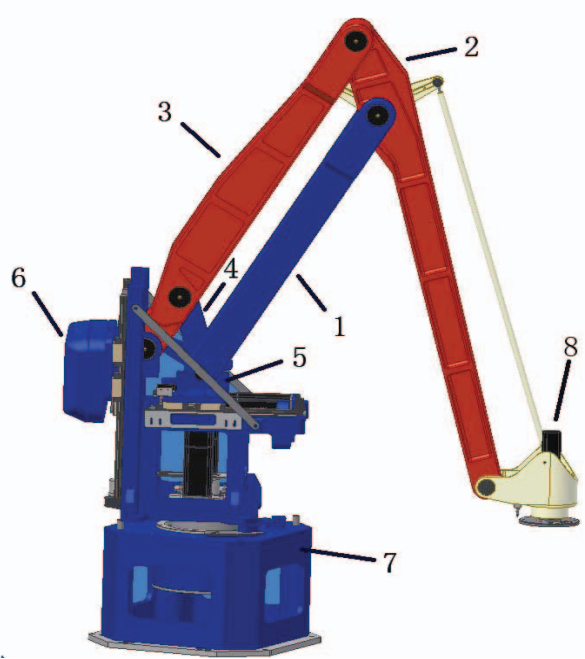
\includegraphics[width=0.4\columnwidth]{alt_robot_arch.png}}
%\hfill
%\subfloat[haptic device with a parallelogram architecture \cite{phantom}.\label{fig:hap_device}]{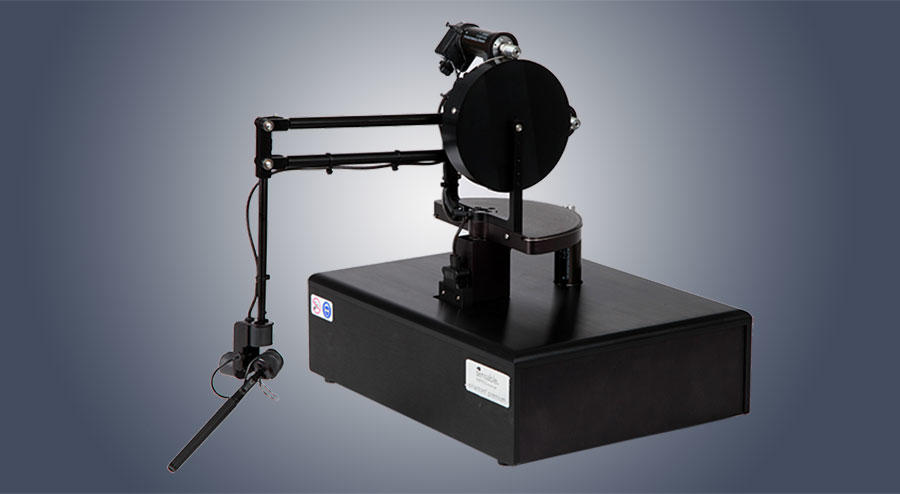
\includegraphics[width=0.5\columnwidth]{phantom.jpg}}

%\subfloat[backdrivable pHRI parallel robot \cite{wen2019kinematically}\cite{9306904}.
%\label{fig:phri_robot}]{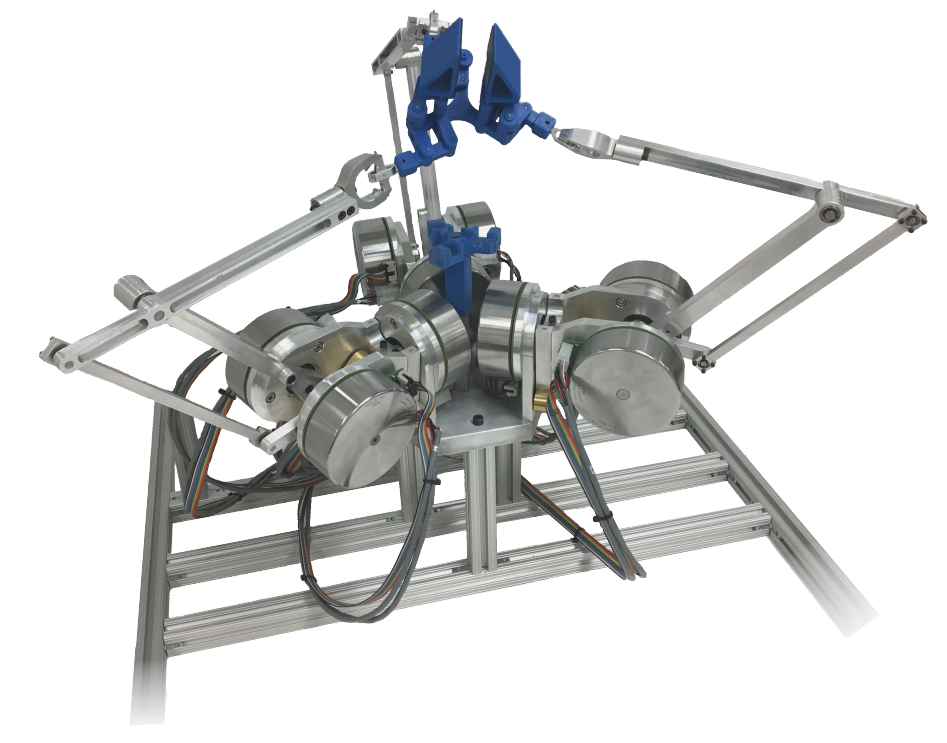
\includegraphics[width=\columnwidth]{proto_keifei.png}}
%\caption{Palletizing robot, haptic device and backdrivable pHRI robot using alternative parallelogram like architectures.}
%\label{fig:alt_arch}
%\end{figure} 
LRT are already used in haptic devices for telesurgery \cite{gosselin2011specification}\cite{perret2014advantages}\cite{baumann1998haptic}\cite{carignan2000closed}. Yet, not all LRT are mechanically backdrivable. For example, a worm gear cannot be driven by its output (through the worm).Table \ref{tab:LRT} shows a list of backdrivable LRT and indicates their advantages and disadvantages for pHRI.
\begin{table}[]
\caption{Comparison of different backdrivable LRT.}
\label{tab:LRT}
\begin{tabularx}{0.5\textwidth}{@{}XXX@{}}
\toprule
LRT type    & Advantages     & Disadvantages                                                                                       \\ \midrule
Spur and helical gears &
  \begin{tabular}[c]{@{}X@{}}High stiffness\\ High torque capability\end{tabular} &
  \begin{tabular}[c]{@{}X@{}}Clearance between\\ teeth\\ (backlash)\end{tabular} \\
\hline
Belt drive &
  \begin{tabular}[c]{@{}X@{}}Transmission over a larger distance\\ No backlash\end{tabular} &
  \begin{tabular}[c]{@{}X@{}}Lower stiffness\\ Slip error\end{tabular} \\
\hline
Chain Drive & High stiffness & \begin{tabular}[c]{@{}X@{}}Clearance between inner links\\ Higher transmission inertia\end{tabular} \\
\hline
Cable (capstan drive) &
  \begin{tabular}[c]{@{}X@{}}Higher stiffness than belt drive\\ No backlash\end{tabular} &
  \begin{tabular}[c]{@{}X@{}}Lower stiffness than chain and gears\\ Slip error\end{tabular} \\ \bottomrule
\end{tabularx}
\end{table}
\par Table \ref{tab:LRT} shows that a capstan drive is a good choice of backdrivable LRT because it has higher stiffness than a belt drive and it has a low backlash like gears or chain drives. This is why it is used in haptic devices \cite{perret2014advantages}\cite{baser2013kinematic}, highly backdrivable collaborative robots \cite{townsend1988effect}\cite{rooks2006harmonious}\cite{phan2014guided} and high precision targeting systems \cite{lu2015development}\cite{lu2012non}\cite{lu2013transmission}\cite{xie2019analytical}. Having low backlash is very important for  robotics applications which require the robot's motors to work in both directions at a high frequency \cite{brooks1990telerobotic}\cite{gealy2019quasi}. However, Table \ref{tab:LRT} also shows that capstan drives have lower stiffness than other LRT such as gears and can be subject to slip error \cite{lu2013transmission}\cite{baser2010theoretical}.\par
In order to alleviate these drawbacks, this article presents a novel capstan architecture that increases the stiffness of the transmission by using grooves on the transmission's pulleys. The grooves increase the friction coefficient between the cable and the pulleys, which makes the transmission stiffer. Moreover, the novel capstan drive allows multiple cable arrangements, which further increases the stiffness of the transmission.\par This paper is structured as follows. In Section II and III, the general modelling of a capstan drive and its torsional stiffness are recalled. The theoretical model used here is based on the work of Werkmeister et al.\cite{werkmeister2007theoretical}. Part of this model is also used in \cite{baser2010theoretical}. Section IV explains how grooves etched along the surface of a capstan drive's pulleys can theoretically increase the friction coefficient between the drive's cable and its pulleys thus increasing the overall stiffness of the capstan drive. The use of grooves in capstan drives has already been presented in \cite{lu2012non}. However, this paper presents a novel design for the output pulley of a capstan drive which uses grooves arranged as a multiple helix. This novel design enables different multi-cable arrangements of the capstan drive that can theoretically further increase its torsional stiffness. The novel capstan drive architecture as well as different possible cable arrangements are presented in Section V. The advantages and disadvantages  of each of the proposed arrangements are discussed. Section VI then proposes a method to properly arrange the capstan drive's pulleys during the drive's assembly so that the cables can follow a smooth and continuous path while passing from one pulley to the other. Finally, concluding remarks are made in Section VIII.
\section{Modelling of a capstan drive}
Figure \ref{fig:model_capstan} presents the different elements of the capstan drive model.
\begin{figure}
    \centering
    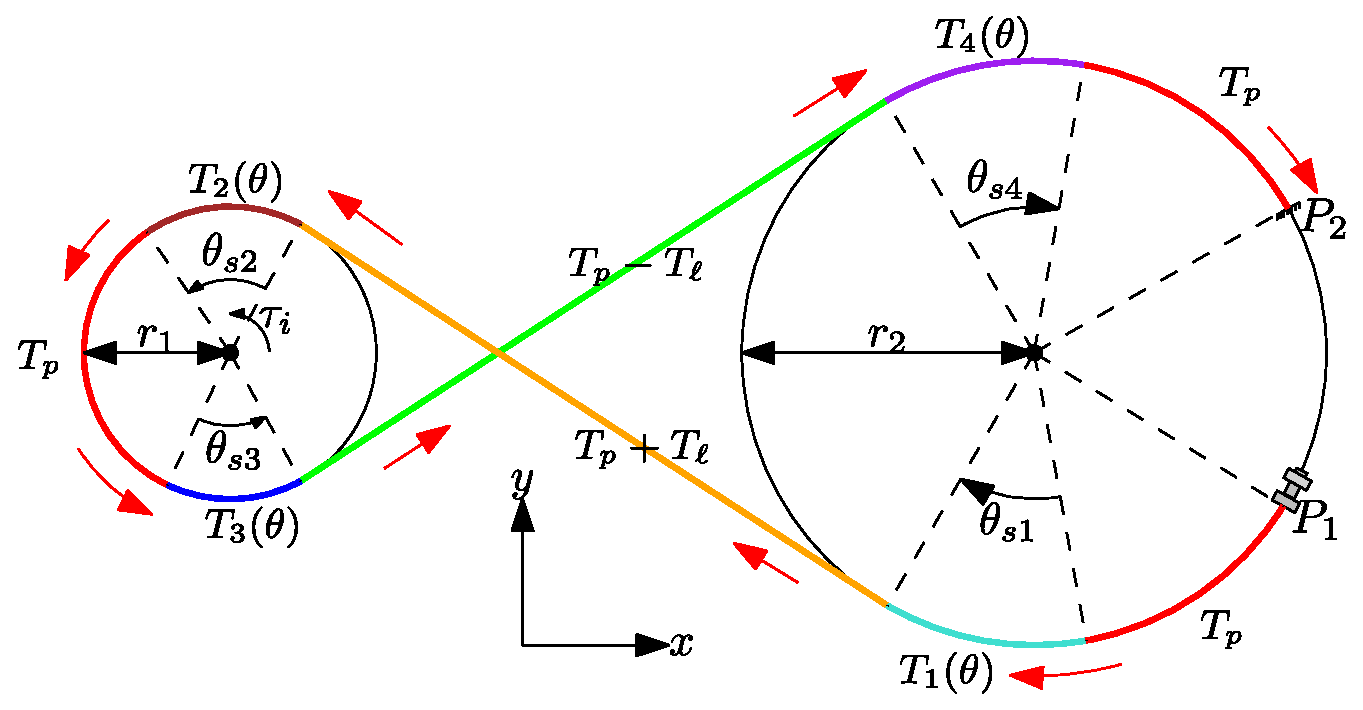
\includegraphics[width=0.46\textwidth]{modelling_of_capstan_drive.eps}
    \caption{Modelling of a capstan drive.}
    \label{fig:model_capstan}
\end{figure}
In figure \ref{fig:model_capstan}, $r_1$ is the radius of the small input pulley while $r_2$ is the radius of the large output pulley. The transmission ratio is given by $R = \frac{r_2}{r_1}$. The cable passes from the large pulley to the small pulley and back to the large pulley in a lemniscate shaped pattern indicated by the red arrows in figure \ref{fig:model_capstan}. A preload tension $T_p$ is applied on the cable by pulling on the cable with a mechanism alike a turnbuckle (at point $P_1$) and by fixing the other end of the cable to the pulley(at point $P_2$).\par
When a torque $\tau_i$ is applied on the input pulley, one side of the cable extends while the other part of the cable shortens. The extension is caused by an increase in the tension in the cable by an amount $T_\ell$ while the contraction of the other part of the cable is caused by a reduction of the tension by an equal amount $T_\ell$. The tension on the taught side becomes $T_p+T_\ell$ while the tension on the loose side becomes $T_p-T_\ell$. The torque balance equation about the axis of rotation of the input pulley can be written as
\begin{align}
    \tau_i - (T_p+T_\ell)r_1 + (T_p-T_\ell)r_1 = 0, \label{eq:first_equation_p0}
\end{align}
which yields
\begin{align}
T_\ell = \frac{\tau_i}{2r_1}.
\label{eq:first_equation}
\end{align}
\par
The tension variations in the cable occur in contact regions between the cable and the pulleys called the slip regions. These regions are represented in figure \ref{fig:model_capstan} with the angles $\theta_{s1}$ to $\theta_{s4}$. Along these slip regions, the cable elongates or shortens due to the applied torque. This local variation in length causes friction between the pulleys and the cable. Figure \ref{fig:friction_fig} illustrates this principle. 
\begin{figure}
    \centering
    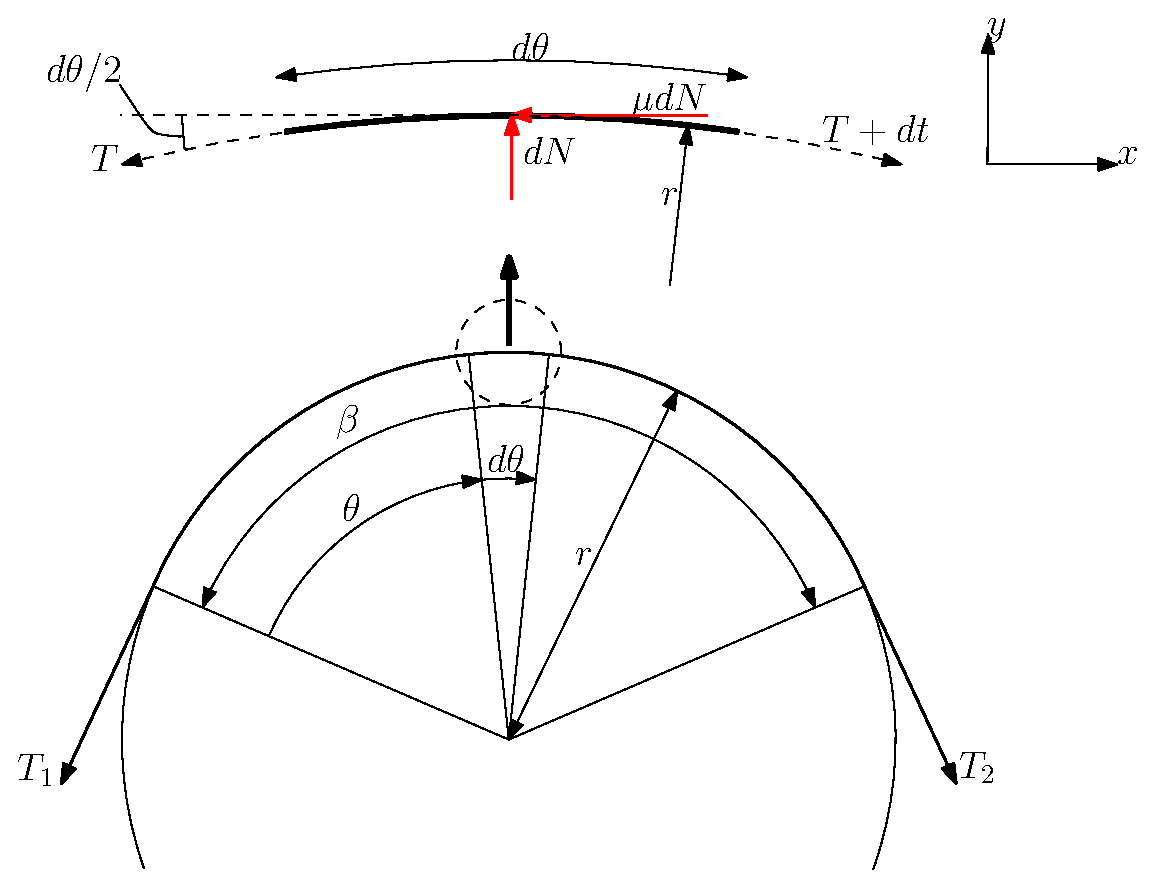
\includegraphics[width = 0.43\textwidth]{capstan_equation.eps}
    \caption{Small segment of the cable pulley interaction.}
    \label{fig:friction_fig}
\end{figure}
\par
Figure \ref{fig:friction_fig} shows a small  segment of a cable lying on the surface of a pulley of radius $r$. The small cable segment is lying on a small angle segment of the pulley $d\theta$. The static friction coefficient between the pulley and the cable is $\mu$. The tension on one end of the small cable segment is $T$ while it is $T+dT$ at the other end. The small tension variation is created by an applied torque on the pulley. The normal force between the small cable segment and the pulley  is $dN$. When torque is applied to the pulley, the pulley surface creates a friction force on the cable segment of $\mu dN$ in the tangential direction of the torque. Calculating the force balance on the cable segment gives 
\begin{align}
    \sum F_x = T\cos\left(\frac{d\theta}{2}\right) - (T+dT)\cos\left(\frac{d\theta}{2}\right) + \mu dN =0,\label{eq:sum_f_x}\\
    \sum F_y = -T\sin\left(\frac{d\theta}{2}\right)-(T+dT)\sin\left(\frac{d\theta}{2}\right)+dN = 0.\label{eq:sum_f_y}
\end{align}
Since $d\theta$ is a small angle and $dT$ is a small tension variation, the following approximations can be made
\begin{align}
    \sin\left(\frac{d\theta}{2}\right)\approx \frac{d\theta}{2},\hquad \cos\left(\frac{d\theta}{2}\right)\approx 1,\hquad dTd\theta \approx 0. 
\end{align}
Applying these approximations to\eqref{eq:sum_f_x} and \eqref{eq:sum_f_y} gives
\begin{align}
    \frac{dT}{T} = \mu d\theta. \label{eq:diff}
\end{align}
In figure \ref{fig:friction_fig}, when the tension varies from $T_1$ to $T_2$ where $T_2>T_1$, the integration over the angle $\beta$ of \eqref{eq:diff} gives
\begin{align} 
\beta = \frac{1}{\mu}\ln\left(\frac{T_2}{T_1}\right).
\label{eq:int_beta}
\end{align}
Angle $\beta$ is referred to as the slip angle of the slip region. Integrating from $T_1$ to a function $T(\theta)$ over the slip region then gives \begin{align}
T(\theta) = T_1e^{\mu\theta},\hquad 0<\theta<\beta.\label{eq:tens_increase}
\end{align}
The same can be said by integrating from the max tension $T_2$ to a smaller tension $T(\theta)$ over the slip region $\beta$, which gives
\begin{align}
T(\theta) = T_2e^{-\mu\theta},\hquad 0<\theta<\beta.\label{eq:tens_decrease}
\end{align}
Applying \eqref{eq:int_beta}, \eqref{eq:tens_increase} and \eqref{eq:tens_decrease} to the slip regions in figure \ref{fig:model_capstan}, one finds
\begin{align}
    T_1(\theta) = T_pe^{\mu\theta},\hquad 0<\theta<\theta_{s1},\hquad \theta_{s1} = \frac{1}{\mu}\ln\left(\frac{T_p+T_\ell}{T_p}\right),\label{eq:Tens1}\\
    T_2(\theta) = (T_p+T_\ell)e^{-\mu\theta},\hquad 0<\theta<\theta_{s2},\hquad \theta_{s2}=\theta_{s1},\label{eq:Tens2}\\
    T_3(\theta) = T_pe^{-\mu\theta},\hquad 0<\theta<\theta_{s3},\hquad \theta_{s3} = \frac{1}{\mu}\ln\left(\frac{T_p}{T_p-T_\ell}\right),\label{eq:Tens3}\\
    T_4(\theta) = (T_p-T_\ell)e^{\mu\theta},\hquad 0<\theta<\theta_{s4},\hquad \theta_{s4} = \theta_{s3}.\label{eq:Tens4}
\end{align}
Equations \eqref{eq:Tens1} to \eqref{eq:Tens4} describe the variation of the tension along the cable. These equations are used in the following section to model the stiffness of a capstan drive.
\section{Stiffness model of a capstan drive}
Hooke's law gives the relationship between the tensile force in an elastic object and its strain. The strain of an elastic object is also defined as its variation in length over its original length. Expressing this definition of strain in an infinitesimal form and equating it to Hooke's law, one can then write
\begin{align}
\epsilon \equiv \frac{d\delta}{dL} = \frac{F}{AE}, \Rightarrow d\delta = \frac{FdL}{AE}
\label{eq:complete_short}
\end{align}
where $\epsilon$ is the strain, $d\delta$ is a very small length variation, $dL$ is a very small cable length, $F$ is the tensile force applied on the elastic object, $A$ is the object's  cross section area and $E$ is its Young modulus. Equation \eqref{eq:complete_short} can be integrated to determine the cable deformation.
\par
The  cable deformation $\delta_i$ along the slip region $\theta_{si}$ is equal to the total deformation along the slip region minus the initial deformation caused by the preload.  Using \eqref{eq:complete_short} and using the fact that $dL=rd\theta$, the deformations $\delta_i$ are obtained as 
\begin{align}
    \delta_i = \frac{r}{AE}\left(\int_0^{\theta_{si}}T_i(\theta)d\theta-T_p\int_0^{\theta_{si}}d\theta\right),\hquad i=1,\ldots ,4 \label{eq:int_deform_i_theta}
\end{align}
where $r = r_2$ for $\theta_{s1}$ and $\theta_{s4}$ and $r = r_1$ for $\theta_{s2}$ and $\theta_{s3}$.
Applying \eqref{eq:int_deform_i_theta} to the slip angle $\theta_{s1}$ gives
\begin{align}
    \delta_1 = \frac{T_pr_2}{AE}\left(\int_0^{\theta_{s1}}e^{\mu\theta} d\theta-\int_0^{\theta_{s1}}d\theta\right), \\
    = \frac{T_pr_2}{AE}\left(\frac{1}{\mu}\left(e^{\mu\theta{s1}} -1\right)-\theta_{s1}\right),\\
    =\frac{r_2}{\mu AE}\left(T_\ell-T_p\ln\left(\frac{T_p+T_\ell}{T_p}\right)\right)\label{eq:defo1}.
\end{align}
Similarly for $\delta_2$ to $\delta_4$, one obtains 
\begin{align}
    \delta_2=\frac{r_1}{\mu AE}\left(T_\ell-T_p\ln\left(\frac{T_p+T_\ell}{T_p}\right)\right),\label{eq:defo2}\\
    \delta_3= \frac{r_1}{\mu AE}\left(T_\ell-T_p\ln\left(\frac{T_p}{T_p-T_\ell}\right)\right),\label{eq:defo3}\\
    \delta_4 =\frac{r_2}{\mu AE}\left(T_\ell-T_p\ln\left(\frac{T_p}{T_p-T_\ell}\right)\right).\label{eq:defo4}
\end{align}
Some cable deformation also occurs in the cable sections which are not in contact with the pulleys. These cable sections are here called the free sections and the deformation along these sections is obtained by integrating \eqref{eq:complete_short} which gives
\begin{align}
\delta_{f1} = \frac{T_p+T_\ell}{AE}\int_0^{L_f}dL=\frac{T_p+T_\ell}{AE}L_f,\label{eq:defof1}\\
\delta_{f2}=\frac{T_p-T_\ell}{AE}\int_0^{L_f}dL=\frac{T_p-T_\ell}{AE}L_f,\label{eq:defof2}
\end{align}
where $\delta_{f1}$ and $\delta_{f2}$ are the deformations on the tight and slack side respectively and $L_f$ is the length of the free parts of the cable which are not in contact with the pulleys.
\par
 The compliance of the different cable sections can be defined as the absolute value of the variation in deformation of the cable as a function of the applied load. Mathematically, this means that the compliance of the different cable sections can be obtained by differentiating the deformation expressions in \eqref{eq:defo1} to \eqref{eq:defof2} with respect to $T_\ell$. Furthermore, since compliance is the inverse of stiffness, one can easily obtain the stiffness of the different cable sections. For the slip regions, this gives
 \begin{align}
     C_{si}=\left|\frac{d\delta_{si}}{dT_\ell}\right|,\hquad i = 1,\ldots ,4,\label{eq:simple_stiff_1}\\
     \Rightarrow C_{s1} = \frac{r_2}{AE\mu}\left(\frac{T_\ell}{T_p+T_\ell}\right) = \frac{1}{K_{s1}}\\
     \Rightarrow C_{s2} = \frac{r_1}{AE\mu}\left(\frac{T_\ell}{T_p+T_\ell}\right)= \frac{1}{K_{s2}}\\
     \Rightarrow C_{s3} =
     \frac{r_1}{AE\mu}\left(\frac{T_\ell}{T_p-T_\ell}\right)= \frac{1}{K_{s3}}\\
     \Rightarrow C_{s4} =
     \frac{r_2}{AE\mu}\left(\frac{T_\ell}{T_p-T_\ell}\right)= \frac{1}{K_{s1}}\label{eq:simple_stiff_4}
 \end{align}
 For the stiffnesses of the free sections of the cable, one obtains
 \begin{align}
     K_{f1}=K_{f2}=\frac{AE}{L_f}
 \end{align}
 The total stiffness of the capstan transmission is obtained by combining the individual stiffnesses of the cable segments along the transmission. The stiffness elements $K_{s1},K_{f_1}$ and $K_{s2}$ form a serial combination of springs. The same can be said for $K_{s3},K_{f_2}$ and $K_{s4}$. The two serial springs groups are in parallel to one another meaning that the total stiffness of the transmission can be written as 
 \begin{align}
     K = K_1 + K_2,
 \end{align}
 where
 \begin{align}
     K_1 = \frac{1}{\frac{1}{K_{s1}}+\frac{1}{K_{f1}}+\frac{1}{K_{s2}}},\\
     K_2 = \frac{1}{\frac{1}{K_{s3}}+\frac{1}{K_{f2}}+\frac{1}{K_{s4}}}.
 \end{align}
 The total stiffness $K$ represents the linear stiffness of the transmission. Since a capstan drive is a torsional element, a better indicator of its stiffness is the drive's torsional stiffness when one of its pulleys is held rigidly. The torsional stiffness $K_t$ of the capstan drive when the small pulley is held rigidly and  a torque $\tau$ is applied on the large pulley, causing an angular displacement $\alpha$, is then given by
 \begin{align}
     \tau = K_t\alpha. \label{eq:rot_stiff}
 \end{align}
 The relationship between $K_t$ and $K$ is obtained by writing
 \begin{align}
    \frac{\tau_D}{r_2} = K\delta \label{eq:lin_stiff}\\
     \alpha = \frac{\delta}{r_2} \label{eq:rot_disp}.
 \end{align}
 Equation \eqref{eq:lin_stiff} gives the relationship between a torque $\tau$ applied on the large pulley  of radius $r_2$ and the total linear displacement $\delta$ when the small pulley is held tightly. Equation \eqref{eq:rot_disp} gives the relationship between the total linear displacement of the cable and the angular displacement $\alpha$ of the large pulley of radius $r_2$. Using these two equations with \eqref{eq:rot_stiff} yields
 \begin{align}
     K_t = Kr_2^2. 
 \end{align}
The following section shows how placing the capstan transmission's cable into grooves helps to increase the coefficient of friction between the cable and the pulleys and therefore the transmission's stiffness.
\section{Influence of grooves on the capstan drive stiffness}
 Analyzing the equations for the stiffness of the different cable sections of a capstan drive ((32) to (35)), one can clearly see that all the stiffness terms are proportional to the coefficient of friction. Therefore, Increasing the coefficient of friction between the cable and the pulleys is an effective way to increase the overall stiffness of the transmission. Figure \ref{fig:distib_force} illustrates how circular grooves help to increase the coefficient of friction between the cable and the capstan drive pulleys.\\
 \begin{figure}
    \centering
    \subfloat[Uniform distribution.\label{fig:uniform_force}]{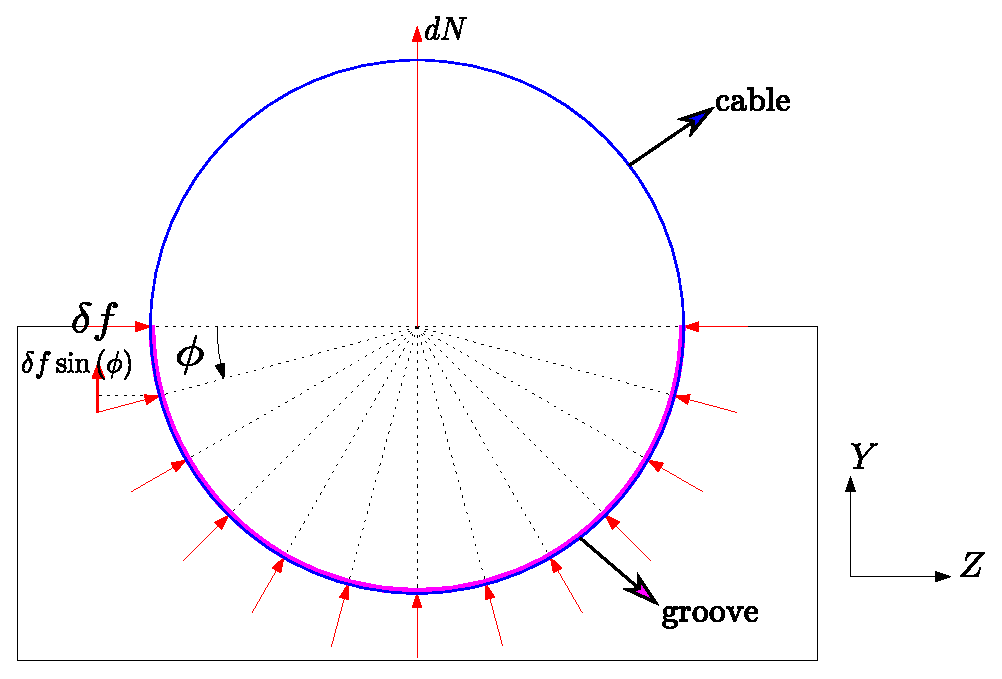
\includegraphics[width =0.8\columnwidth]{distribution_de_force_cable.eps}}
    
    \subfloat[General distribution.\label{fig:general_force}]{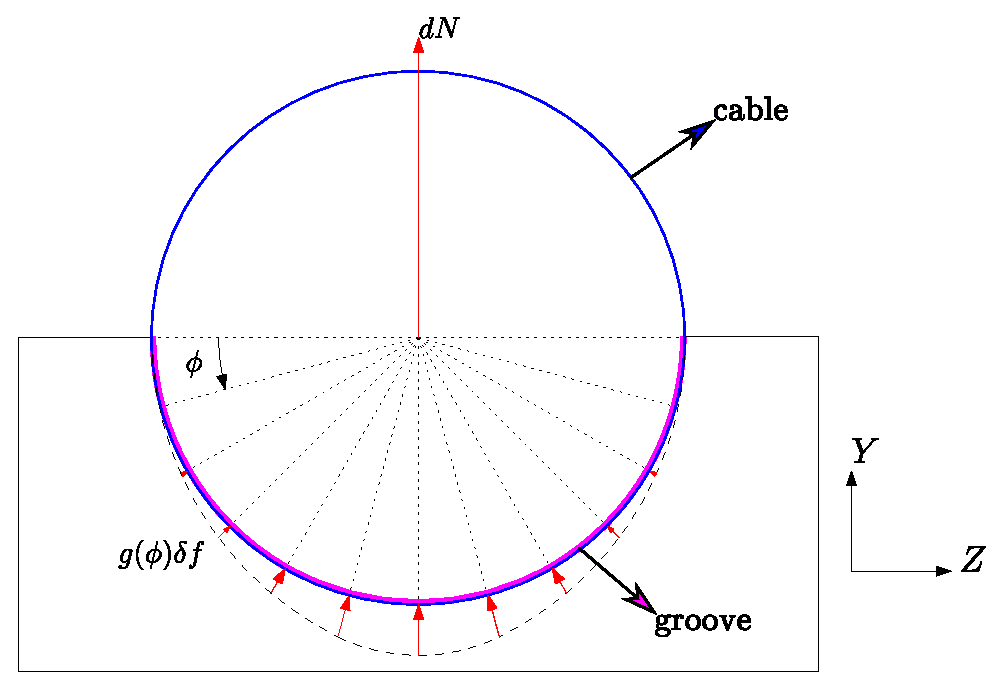
\includegraphics[width =0.8\columnwidth]{distribution_tension_gen.eps}}
    \caption{Distribution of the normal force along the cross-section interface between the cable and the pulleys.}
    \label{fig:distib_force}
\end{figure}
 The illustrations in figure \ref{fig:distib_force} show the distribution of the normal force occurring between a small section of the cable and a pulley groove. In figure \ref{fig:uniform_force}, the distribution of the normal force is considered to be uniform along the interface between the cable and the groove. The figure shows the cross section of the interface which is perpendicular to the plane shown in figure \ref{fig:friction_fig}. The equivalent normal force between the small cable segment and the pulley segment is noted $dN$ and can be mathematically obtained as 
 \begin{align}
     dN = \int_0^\pi \delta f\sin{\phi}d\phi = 2\delta f,
     \label{eq:small_normforce}
 \end{align}
 where $\phi$ is the variable angle along the interface cross section and $\delta f$ is a unit force quantity. Applying Coulomb's law of static friction to the cross-section in figure \ref{fig:uniform_force} gives 
 \begin{align}
     dF_f = \int_0^\pi\mu df d\theta=\pi\mu df, \label{eq:small_friction}
 \end{align}
 where $dF_f$ is the friction force between the cable segment and the cable pulley. Combining  \eqref{eq:small_normforce} and \eqref{eq:small_friction} gives
 \begin{align}
     dF_f=\mu'dN=\frac{\pi\mu}{2}dN,\label{eq:eff_fric}
 \end{align}
 where $\mu'$ is the effective coefficient of friction between the cable and the pulley grooves. Equation \eqref{eq:eff_fric} shows that, when considering a uniform distribution along the cross section of the cable pulley interface, grooves can help to increase the effective friction coefficient by a factor of $\pi/2$. However, this force distribution along the interface arc is very unlikely considering the fact that local normal force around the middle of the cross-section arc is likely larger than the one at each extremity of the cross-section arc. Considering this, figure \ref{fig:general_force} shows how the force could be distributed along the cross-section arc if a general force distribution function $g(\phi)$ is considered. The effective friction coefficient given this consideration is then obtained by
 \begin{align}
     dN = \delta f I_1(\phi) = \delta f\int_0^{\pi}g(\phi)\sin\phi d\phi,\\
     dF_f = \mu\delta f I_2(\phi) = \mu\delta_f\int_0^\pi\mu g(\phi)d\phi.\\
     dF_f =\mu'dN= \frac{\mu I_2(\phi)}{I_1(\phi)}dN.
 \end{align}
 For any type of positive distribution function $g(\phi)$, the ratio of $\frac{I_2(\phi)}{I_1(\phi)}$ will always be greater than 1. This means that a groove can only increase the effective friction coefficient between the cable and the pulleys of a capstan drive and will therefore make it stiffer. 
\\ 
 The following section presents a novel capstan drive architecture that takes advantage of the increased effective friction coefficient of grooved pulleys and uses multiple grooves on its output pulley in order to allow different cable arrangements which further increase the stiffness of the drive.
  \section{Novel capstan drive architecture}
 The novel architecture is presented in figure \ref{fig:novel_arch}. The novel capstan drive is composed of two pulleys, the input pulley of radius $r_1$ which is connected to the motor and the output pulley of radius $r_2$ which is connected to the output of the drive.  A cable indicated by a red line goes from the output pulley to the input pulley and back to the output pulley. Points $P_1$ and $P_2$ are anchoring points where the cable is fixed. The grooves on each pulley have identical cross sections. However, the groove on the input pulley forms a single helix with a pitch of $H_1$ while the grooves on the output pulley form a R-helix where $R$ is the reduction ratio of the drive, i.e. $r_2/r_1$. In figure \ref{fig:novel_arch}, the grooves on the output pulley are each indicated with a different colour to help differentiate them. Each of the output grooves has a pitch of $H_2$, where $H_2 = RH_1$.
 \begin{figure}
     \centering
     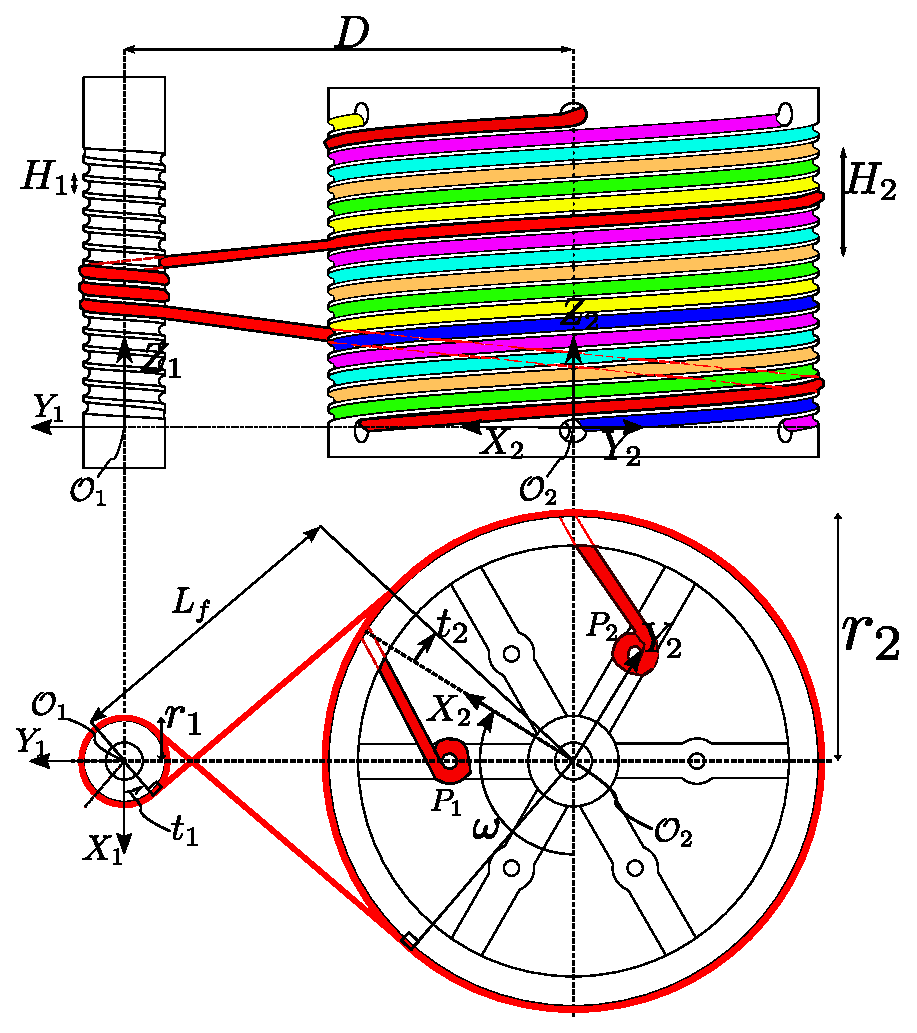
\includegraphics[width =0.8\columnwidth]{test_print_poulies.eps}
     \caption{Architecture of the novel capstan drive.}
     \label{fig:novel_arch}
 \end{figure}
 The grooves of the output pulley evolve in a direction opposite that of the grooves of the input pulley. The free cable length $L_f$ indicates the part of the cable that is not in direct contact with either of the drive pulleys. The distance between the centre axes of the pulleys is noted $D$. \\
 The presence of grooves on both the input and the output pulleys helps to increase the stiffness of the drive by increasing the effective coefficient of friction between the cable and the pulleys, as mentioned in the preceding section. Furthermore, the multiple grooves present on the output pulley enable the use of multiple cables in different cable arrangements, which can further increase the stiffness of the drive.\\
Figure \ref{fig:cable_arrangements} illustrates the different possible cable arrangements. 
 \begin{figure*}
    \centering
    \subfloat[One cable fixed at both ends to the output pulley.\label{fig:single_cable_multi_loops}]
    {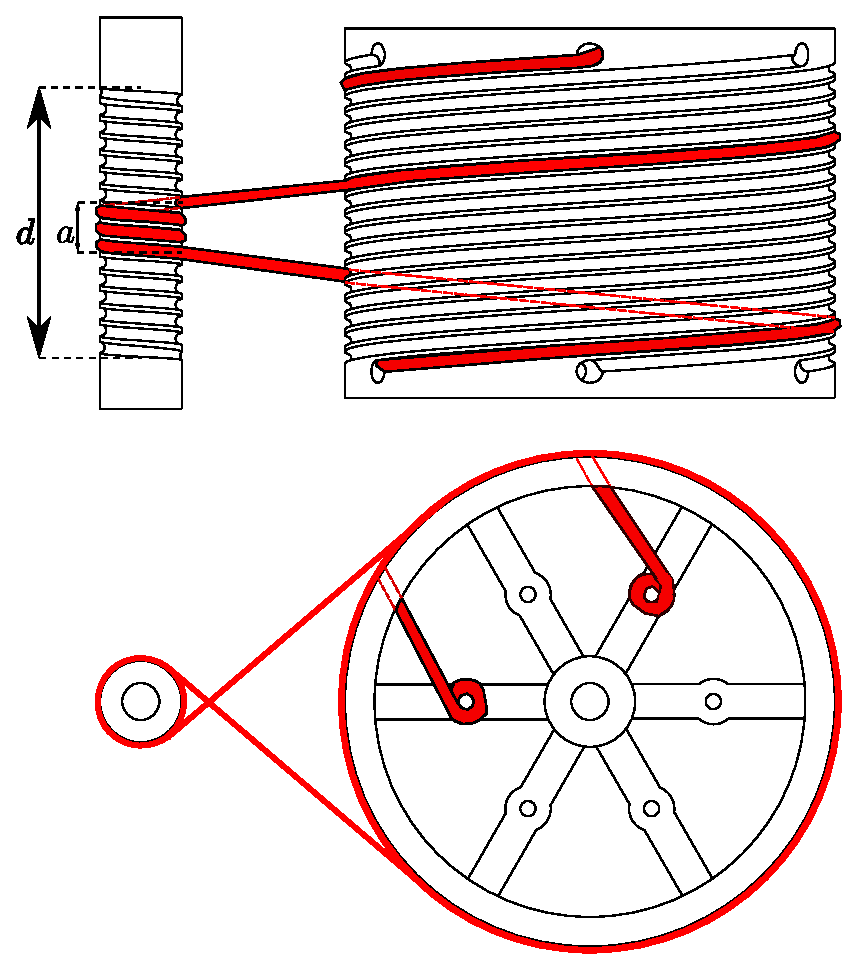
\includegraphics[width =0.54\columnwidth]{only_one_cable_multi_loops.eps}}\hspace{0.1\textwidth}
    \subfloat[Two cables both fixed at both ends to the output pulley.\label{fig:2cables_multi_loops}]{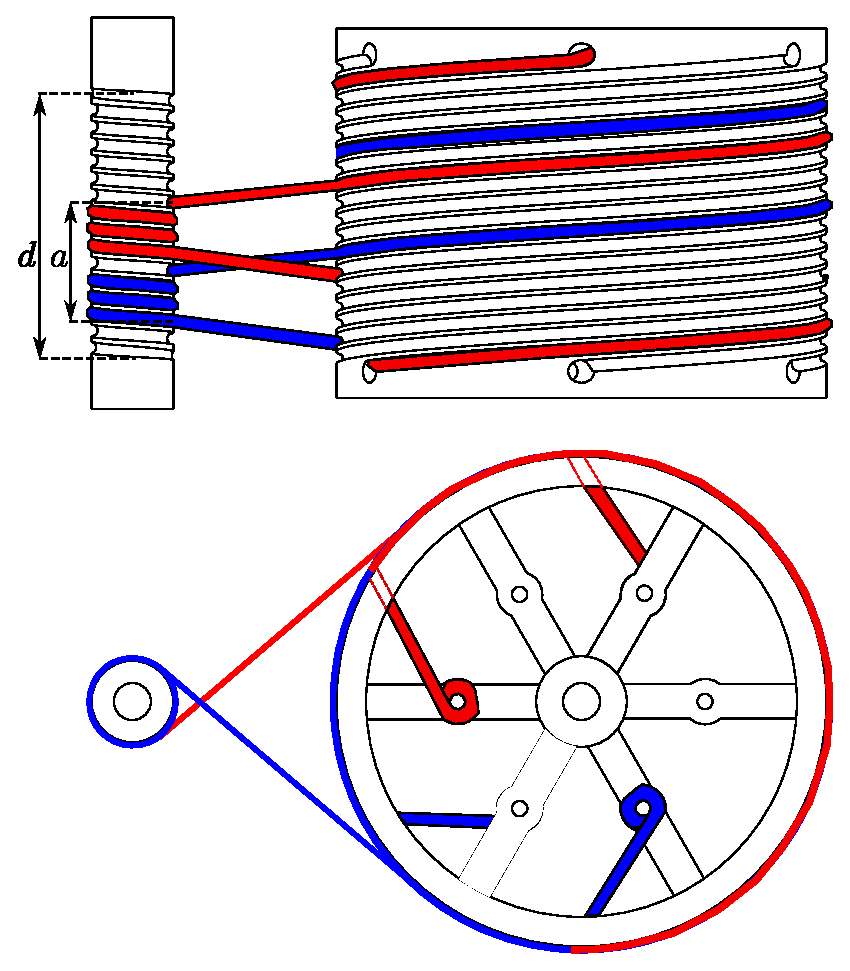
\includegraphics[width=0.54\columnwidth]{two_cables_multi_loops.eps}}
    
    \subfloat[Two cables with ends fixed at the input pulley and the output pulley.\label{fig:multi_cables_full_loops}]{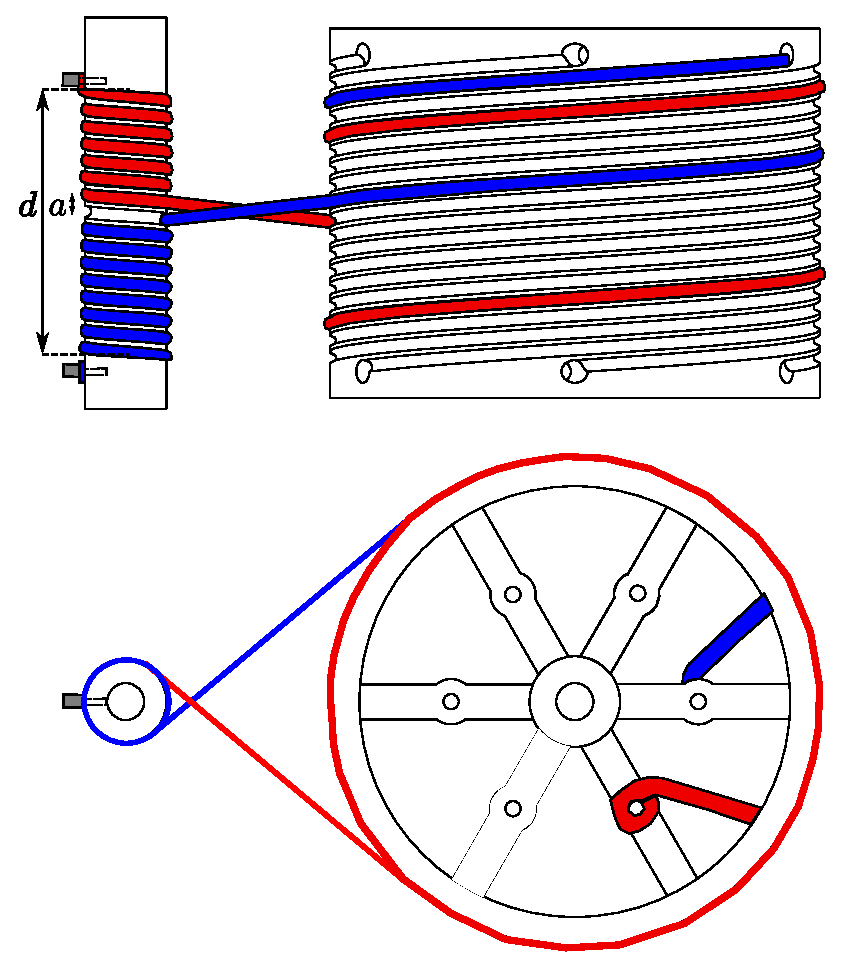
\includegraphics[width=0.54\columnwidth]{two_cables_all_loops.eps}}\hspace{0.1\textwidth}
    \subfloat[Three cables, two having ends fixed at the input and output pulley and one being fixed at both ends to the output pulley.\label{fig:three_cables_multi_loops}]{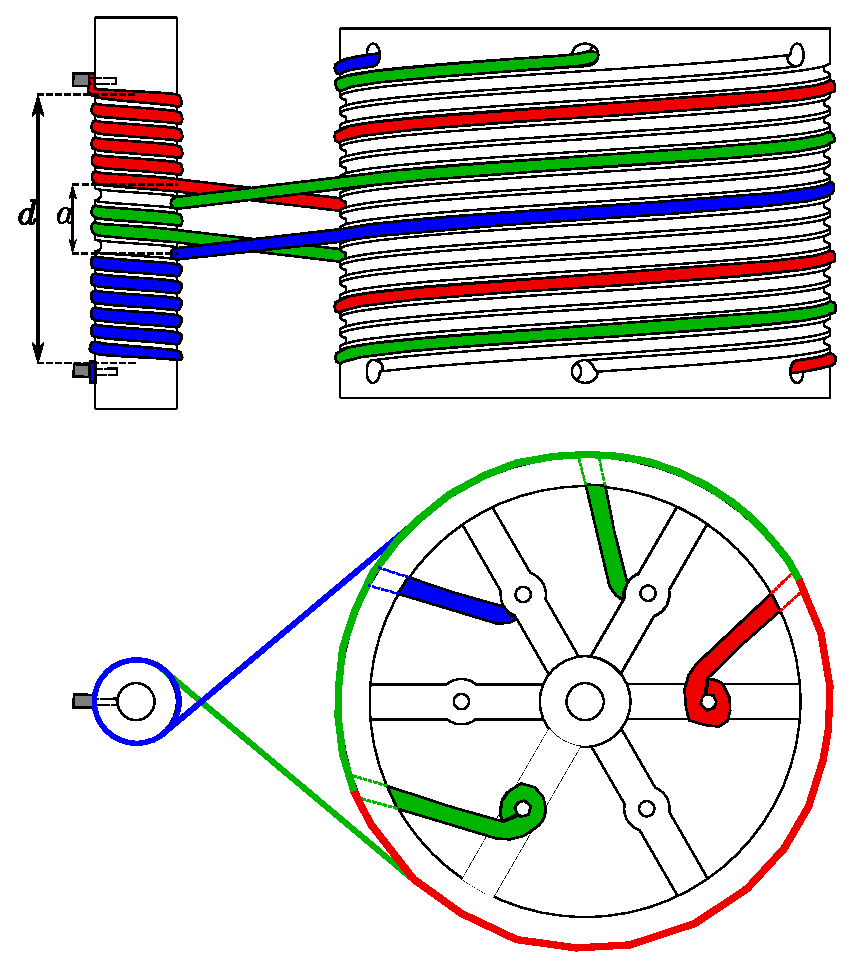
\includegraphics[width=0.54\columnwidth]{three_cables_multi_loops.eps}}
    \caption{Different possible cable arrangements.}
    \label{fig:cable_arrangements}
\end{figure*}
In figure \ref{fig:single_cable_multi_loops}, a single cable is used which is fixed at both ends to the output pulley. This arrangement has the advantage of being simple and its stiffness model is equivalent to the stiffness model of a typical capstan drive such as the one presented in figure \ref{fig:model_capstan}. This arrangement can be used many times in parallel as shown in figure \ref{fig:2cables_multi_loops} in order to multiply the total stiffness of the transmission. However, since none of the cables are fixed to the input pulley, slipping of the input pulley is possible.\\
The layout shown in figure \ref{fig:multi_cables_full_loops} uses two cables. Each cable is fixed to the input pulley at one end and to the output pulley at the other end. This cable arrangement has the advantage of ensuring that the input pulley does not slip. However, it requires two cables to obtain a transmission stiffness which is equivalent to the transmission stiffness of a single cable arrangement in figure \ref{fig:single_cable_multi_loops}.\\
The layout shown in figure  \ref{fig:three_cables_multi_loops} uses three cables. Two of its cables are fixed to both the input and output pulley while its third cable is strictly fixed to the output pulley but loops over the input pulley. The first two cables ensure the motion coupling of the input and output pulley (that there is no slipping) while the third cable helps to increase the transmission stiffness. This cable arrangement has the advantages of the two previous arrangements. \\
In all the cable arrangements shown in figure \ref{fig:cable_arrangements}, the number of turns that can be made by the output pulley is given by 
\begin{align}
N = \frac{d-a}{H_1R},
\end{align}
where  $d$ and $a$ are defined in figure \ref{fig:cable_arrangements}, $H_1$ is the pitch of the groove on the input pulley and $R$ is the reduction ratio of the drive.
In order for the cables to pass from the input pulley to the output pulley and vice versa, geometric conditions must be met in order to ensure that the helical path described by the input groove aligns with one of the helical paths of the output pulley grooves. The following section presents a mathematical model that ensures proper alignment.
\section{Alignment of the input and output grooves}
 The groove on the input pulley can best be described as a helix. The parametric helix function of the groove on the input pulley is given by 
 \begin{align}
     \mathbf{p}_1(t_1) = \begin{bmatrix}
     r_1\cos t_1\\-r_1\sin t_1\\\frac{H_1t_1}{2\pi}
     \end{bmatrix}
     \label{eq:helix_1nput}
 \end{align}
  with respect to the reference frame of the input pulley $\mathcal{O}_1$. The $X_1$ axis of $\mathcal{O}_1$ points towards the starting point of the helix. In \eqref{eq:helix_1nput},
 $t_1$ is the helix parameter of the trajectory. The second term of $\mathbf{p}_1(t_1)$ has a negative sign since the helix on the input pulley evolves in a direction opposite to the reference frame $\mathcal{O}_1$. Differentiating $\mathbf{p}_1(t_1)$ with respect to $t_1$ gives a vector that is tangent to $\mathbf{p}_1(t_1)$ and which can be written as
 \begin{align}
     \mathbf{q}_1(t_1) = \frac{d\mathbf{p}_1(t_1)}{dt_1} = \begin{bmatrix}
     -r_1\sin t_1\\-r_1\cos t_1\\\frac{H_1}{2\pi}
     \end{bmatrix} 
 \end{align}
 The unit vector $\mathbf{u}_1(t_1)$ along $\mathbf{q}_1(t_1)$ is obtained by dividing $\mathbf{q}_1(t_1)$ by its Euclidean norm which gives
 \begin{align}
     \mathbf{u}_1(t_1) = \frac{\mathbf{q}_1(t_1)}{\rho_1}, \hquad \rho_1 = \frac{\sqrt{H_1^2+4\pi^2r_1^2}}{2\pi}.
 \end{align}
  The grooves on the output pulley can also be described by parametric helix functions. These functions can be written as
  \begin{align}
      \mathbf{p}_{2i}(t_{2i}) = \begin{bmatrix}
      r_2\cos t_{2i}\\
      r_2\sin t_{2i}\\
      \frac{H_2 t_{2i}}{2\pi}
      \end{bmatrix},\\ t_{2i} = t_2+\frac{(i-1)}{R}2\pi, \hquad i =1 ,\ldots , R,
      \label{eq:output_helix}
  \end{align}
  with respect to the reference frame of the output pulley $\mathcal{O}_2$. The $X_2$ axis points towards the starting point of one of the output grooves. In \eqref{eq:output_helix}, $t_2$ is the general helix parameter of the output pulley and the $t_{2i}$ parameters are specific to each individual groove of the output pulley. \\ 
  Differentiating vectors $\mathbf{p}_{2i}(t_{2i})$ with respect to $t_{2}$ gives vectors that are tangent to their respective $\mathbf{p}_{2i}(t_{2i})$ vectors. These tangent vectors can be written as 
  \begin{align}
      \mathbf{q}_{2i}(t_{2i}) = \frac{d \mathbf{p}_{2i}(t_{2i})}{dt_{2}}=\begin{bmatrix}
      -r_2\sin t_{2i}\\
      r_2\cos t_{2i}\\
      \frac{H_2}{2\pi}
      \end{bmatrix},\hspace{0.5em}i =1 ,\ldots , R.
  \end{align}
  The tangent unit vectors along the $\mathbf{q}_{2i}(t_{2i})$ vectors are given by
  \begin{align}
      \mathbf{u}_{2i}(t_{2i}) = \frac{\mathbf{q}_{2i}}{\rho_2},\hspace{0.5em} \rho_2 = \frac{\sqrt{H_2^2+4\pi^2r_2^2}}{2\pi}, \hspace{0.5em} i = 1 ,\ldots , R.
  \end{align}
  The helix functions of the input pulley groove and one of the output pulley grooves can be expressed as a function of one another in the following loop closure equation
  \begin{align}
      \mathbf{p}_1 + L_f\mathbf{u}_1 = \mathbf{a}+\mathbf{Q}\mathbf{p}_{2i}, \hquad i =1 ,\ldots , R,
      \label{eq:loop_closure}
  \end{align}
  where $\mathbf{a}=\begin{bmatrix}0 && -D  && 0\end{bmatrix}^T$ is a vector expressed in the $\mathcal{O}_1$ reference frame and $\mathbf{Q}$ is a rotation matrix expressing a change of reference frame from $\mathcal{O}_2$ to $\mathcal{O}_1$ and is written as \begin{align}
  \mathbf{Q} =
  \begin{bmatrix}
  \cos \omega && -\sin \omega && 0\\
  \sin \omega && \cos \omega && 0\\
  0 && 0 && 1
  \end{bmatrix},
  \end{align}
  where $\omega$ represents the amount of rotation of the output pulley needed in order to have the cables pass smoothly between the two pulleys.
  Equation \eqref{eq:loop_closure} is equivalent to the three following scalar equations
  \begin{equation}
  \begin{multlined}
      r_1\left(\cos t_1 -\frac{L_f}{\rho_1}\sin t_1\right)=r_2\cos\left(\omega+t_{2i}\right),\\ i=1 ,\ldots , R,\label{eq:loop_closure_deriv1}
      \end{multlined}
      \end{equation}
      \begin{align}
      \begin{multlined}
      -r_1\left(\sin t_1 + \frac{L_f}{\rho_1}\cos t_1\right)=-D+r_2\sin\left(\omega+t_{2i}\right),\\ i=1 ,\ldots , R,\label{eq:loop_closure_deriv2}
      \end{multlined}
      \end{align}
      \begin{equation}
      H_1\left(t_1+\frac{L_f}{\rho_1}\right) = H_2t_2.\label{eq:loop_closure_deriv3}
  \end{equation}
  In addition to these equations, in order to ensure the proper alignment of the input and output pulley grooves, one must be able to draw a straight line from the input groove to one of the output grooves where the line is tangent to both grooves. This can be mathematically written as 
  \begin{align}
      \mathbf{q}_1 \times \mathbf{Q}\mathbf{q}_{2i} = \mathbf{0},\hquad i=1 ,\ldots , R,
  \end{align}
  which is equivalent to the following three scalar equations 
  \begin{align}
      \frac{H_2r_1}{2\pi}\cos t_1 + \frac{H_1r_2}{2\pi}\cos(\omega+t_{2i})=0,\hquad i=1 ,\ldots , R,\label{eq:cross_prod_1}\\
      \frac{H_2r_1}{2\pi}\sin t_1-\frac{H_1r_2}{2\pi}\sin(\omega + t_{2i})=0,\hquad i=1 ,\ldots , R,\label{eq:cross_prod_2}\\
      \sin\left(t_1+t_{2i}+\omega\right)=0,\hquad i=1 ,\ldots , R.\label{eq:cross_prod_3}
  \end{align}
From \eqref{eq:cross_prod_3}, we obtain that
\begin{align}
    t_1+t_{2i}+\omega = n\pi, n\in \mathbb{N},\hquad i = 1,\ldots ,R.\label{eq:cross_prod_deriv1}
\end{align}
Substituting \eqref{eq:cross_prod_deriv1} into \eqref{eq:cross_prod_1} and \eqref{eq:cross_prod_2} yields
\begin{align}
    \frac{H_2r_1}{2\pi}\cos t_1 + \frac{H_1r_2}{2\pi}\cos(n\pi-t_1)=0,\hquad i=1,\ldots ,R,\label{eq:cross_prod_deriv2}\\
    \frac{H_2r_1}{2\pi}\sin t_1-\frac{H_1r_2}{2\pi}\sin( n\pi-t_1)=0,\label{eq:cross_prod_deriv3}\hquad i=1 ,\ldots , R.
\end{align}
Equations \eqref{eq:cross_prod_deriv2} and \eqref{eq:cross_prod_deriv3} are both satisfied if 
\begin{align}
    H_2r_1 = H_1r_2\label{eq:cond_cross_prod_2}
\end{align} 
and 
\begin{align}
    n = 2m+1, \hquad m \in \mathbb{N}.\label{eq:cond_cross_prod_3}
\end{align}
Equations \eqref{eq:cross_prod_deriv1}, \eqref{eq:cond_cross_prod_2} and \eqref{eq:cond_cross_prod_3} represent the conditions that must be met in order to be able to draw a straight line from the input pulley groove to one of the output pulley grooves where the line is tangent to both grooves. Substituting these conditions into \eqref{eq:loop_closure_deriv1} and \eqref{eq:loop_closure_deriv3} leads to
\begin{align}
    (r_2+r_1)\cos t_1 = \frac{L_fr_1}{\rho_1}\sin t_1,\label{eq:loop_closure_deriv4}\\
    D - \left(r_2+r_1\right)\sin t_1 = \frac{L_fr_1}{\rho_1}\cos t_1.\label{eq:loop_closure_deriv5}
\end{align}
Dividing  \eqref{eq:loop_closure_deriv4} by \eqref{eq:loop_closure_deriv5} and rearranging then yields
\begin{align}
   \sin t_1 = \left(\frac{r_2+r_1}{D}\right).\label{eq:deriv_eq_tI}
\end{align}
The right-hand side term in \eqref{eq:deriv_eq_tI} is bound between 0 and 1 since $D\in\left[(r_2+r_1),\infty \right[$. This means that 
\begin{align}
    t_1 =  \varphi + 2\pi p,\hquad p \in \mathbb{N}\label{eq:deriv_eq_tI2}
\end{align}
or 
\begin{align}
    t_1 =(2p+1)\pi-\varphi,\hquad p \in \mathbb{N},\label{eq:deriv_eq_tI3}\\
    \varphi = \sin^{-1}\left(\frac{r_1+r_2}{D}\right).
\end{align}
Substituting \eqref{eq:deriv_eq_tI3} into \eqref{eq:loop_closure_deriv4}, one finds that $L_f$ would need to have a negative length, which is impossible. This is not the case when $t_1$ is given by \eqref{eq:deriv_eq_tI2} and therefore this is the only possible value for $t_1$. The value of $L_f$ is thus
\begin{align}
L_f = \frac{\rho_1}{r_1}\sqrt{D^2-(r_2+r_1)^2}.
\label{eq:val_Lf}
\end{align}
Having $L_f$ and $t_1$, one can finally find the value of $\omega$ using \eqref{eq:loop_closure_deriv3} and \eqref{eq:cross_prod_deriv1} as 
\begin{align}
\begin{multlined}
\omega = \left(2m+1\right)\pi-t_1-\frac{\left(t_1+\frac{L_f}{\rho_1}\right)}{R}-\frac{2\pi(i-1)}{R},\\ i=1 ,\ldots , R, m \in \mathbb{N},
\label{eq:delta_def}
\end{multlined}
\end{align}
with $t_1$ given by \eqref{eq:deriv_eq_tI2} and $L_f$ given by \eqref{eq:val_Lf}. Equation \eqref{eq:delta_def} can be simplified since the output pulley is $2\pi/R$ symmetric about the $Z_2$ axis in figure \ref{fig:novel_arch}. The simplified version of \eqref{eq:delta_def} is written as
\begin{align}
\omega = \left(\frac{-\left(\varphi\left(R+1\right)+\frac{L_f}{\rho_1}\right)}{R}\right)//\left(\frac{2\pi}{R}\right),
\end{align}
where $a//b$ returns the remainder of $a$ divided by $b$.\\

Angle $\omega$ varies with the distance separating the axes of the input and output pulleys $D$. Knowing $D$, properly aligning the pulleys so that the cables follow a smooth path simply requires that both pulleys be locked during the cable mounting with the large pulley being rotated by an angle $\omega$ from the $X_1$ axis of the small pulley around the $Z_2$ axis of the large pulley. After having taught all the cables at both ends, the system can then be unlocked and the pulley grooves are properly aligned. This process is better illustrated in figure \ref{fig:process_align}.
\begin{figure*}
\centering
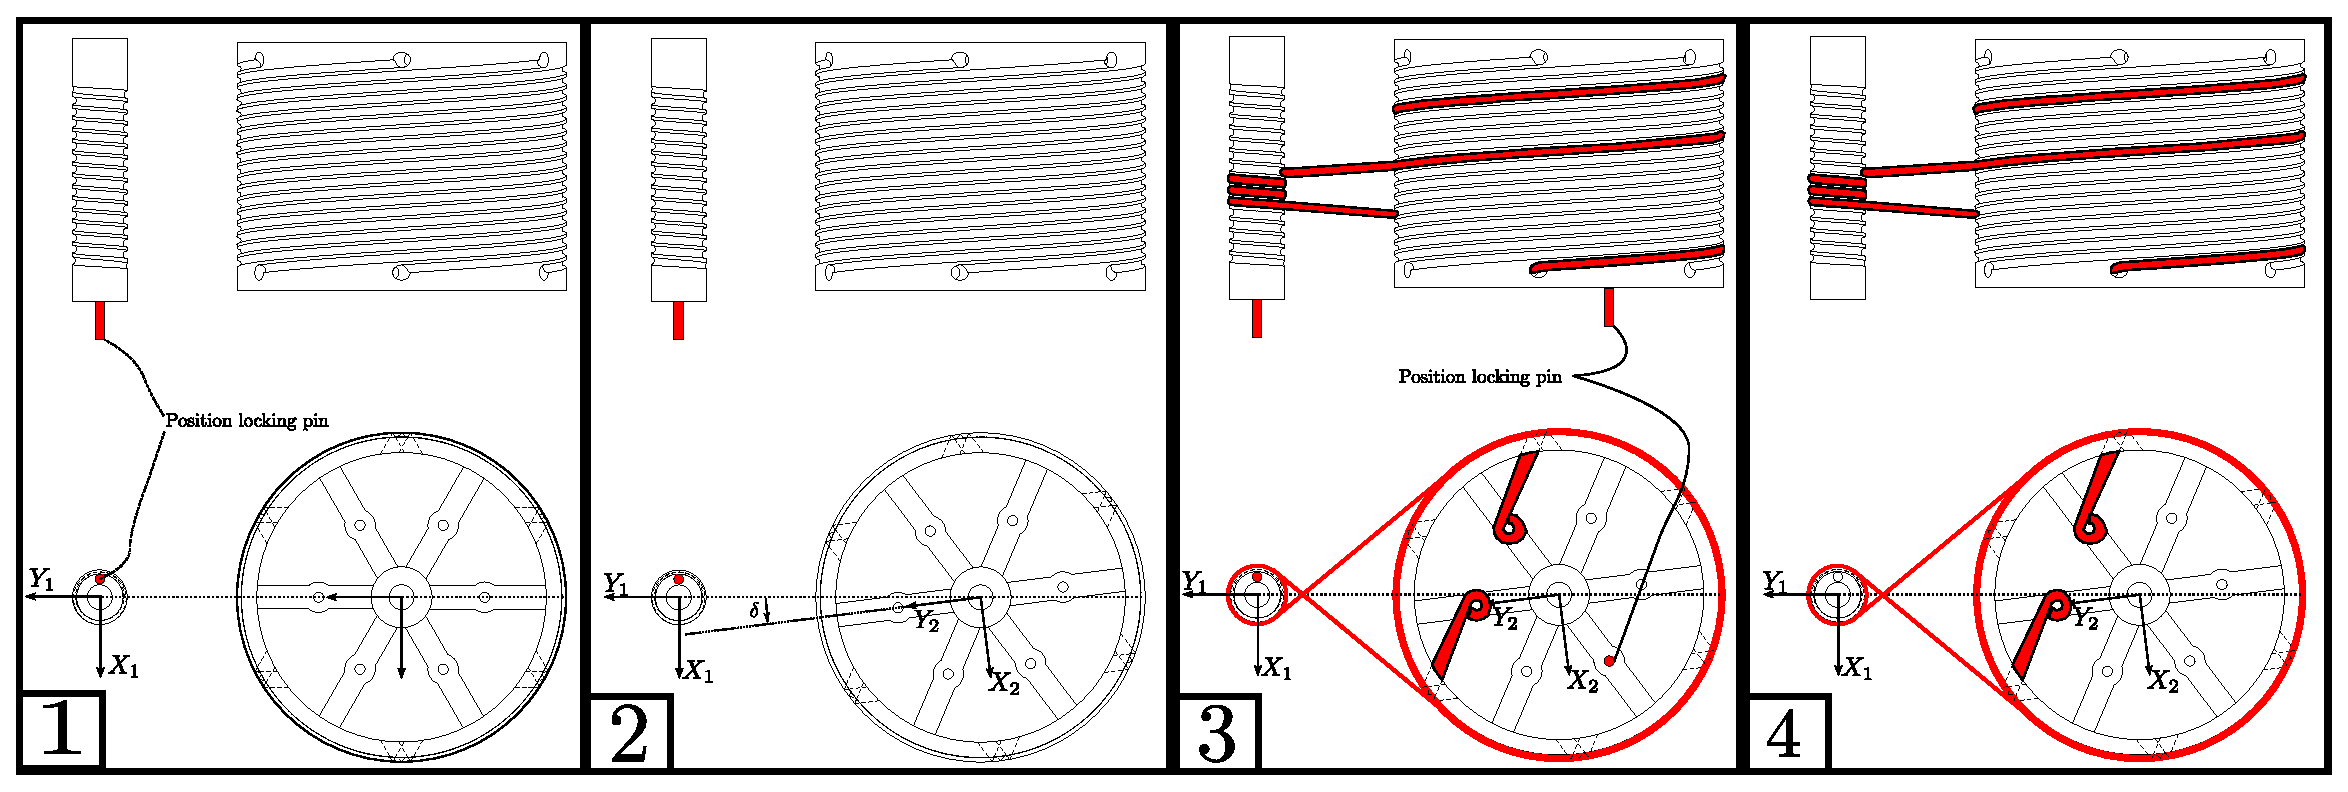
\includegraphics[width = \textwidth]{steps.eps}
\caption{Steps to align the drive pulleys for smooth cable trajectories.}
\label{fig:process_align}
\end{figure*}
\section{Multimedia extension}
A video accompanies this paper. The video demonstrates the operation of a prototype of the novel capstan drive as well as its backdrivability.
\section{Conclusion}
This paper presented a novel capstan drive architecture which uses grooves on both its input and output pulleys in order to increase the effective coefficient of friction between the drive cables and the pulleys. Using a previously established model of a capstan drive, it was shown that increasing the coefficient of friction between the drive cables and the drive pulleys increases the drive stiffness, which is an important property in several applications, including for instance physical human-robot interaction. Furthermore, the many grooves on the output pulley enable multi-cable arrangements which can even further increase the transmission's stiffness. A method to ensure that the drive cables can pass smoothly between the input and output pulley was also described. \\
Future work on this novel capstan drive will consist in testing the established model in a test bench in order to quantify the increased coefficient of friction caused by the grooves as well as to quantify the increase in drive stiffness compared to a standard capstan drive. Furthermore, the influence of the increased drive stiffness on the drive's bandwidth will be analyzed and compared to other small-ratio transmissions in order to determine if this novel drive is advantageous for physical human robot interaction.
\section*{Acknowledgments}
The financial support of the Natural Sciences and Engineering Research Council of Canada (NSERC) and of the Canada Research Chair program is gratefully acknowledged.

\bibliographystyle{./bibliography/IEEEtran}
\bibliography{./bibliography/asme2e}
%\begin{IEEEbiography}{Michael Shell}
%Biography text here.
%\end{IEEEbiography}

% if you will not have a photo at all:
%\begin{IEEEbiographynophoto}{John Doe}
%Biography text here.
%\end{IEEEbiographynophoto}

% insert where needed to balance the two columns on the last page with
% biographies
%\newpage

%\begin{IEEEbiographynophoto}{Jane Doe}
%Biography text here.
%\end{IEEEbiographynophoto}
% An example of a floating figure using the graphicx package.
% Note that \label must occur AFTER (or within) \caption.
% For figures, \caption should occur after the \includegraphics.
% Note that IEEEtran v1.7 and later has special internal code that
% is designed to preserve the operation of \label within \caption
% even when the captionsoff option is in effect. However, because
% of issues like this, it may be the safest practice to put all your
% \label just after \caption rather than within \caption{}.
%
% Reminder: the "draftcls" or "draftclsnofoot", not "draft", class
% option should be used if it is desired that the figures are to be
% displayed while in draft mode.
%
%\begin{figure}[!t]
%\centering
%\includegraphics[width=2.5in]{myfigure}
% where an .eps filename suffix will be assumed under latex, 
% and a .pdf suffix will be assumed for pdflatex; or what has been declared
% via \DeclareGraphicsExtensions.
%\caption{Simulation results for the network.}
%\label{fig_sim}
%\end{figure}

% Note that the IEEE typically puts floats only at the top, even when this
% results in a large percentage of a column being occupied by floats.


% An example of a double column floating figure using two subfigures.
% (The subfig.sty package must be loaded for this to work.)
% The subfigure \label commands are set within each subfloat command,
% and the \label for the overall figure must come after \caption.
% \hfil is used as a separator to get equal spacing.
% Watch out that the combined width of all the subfigures on a 
% line do not exceed the text width or a line break will occur.
%
%\begin{figure*}[!t]
%\centering
%\subfloat[Case I]{\includegraphics[width=2.5in]{box}%
%\label{fig_first_case}}
%\hfil
%\subfloat[Case II]{\includegraphics[width=2.5in]{box}%
%\label{fig_second_case}}
%\caption{Simulation results for the network.}
%\label{fig_sim}
%\end{figure*}
%
% Note that often IEEE papers with subfigures do not employ subfigure
% captions (using the optional argument to \subfloat[]), but instead will
% reference/describe all of them (a), (b), etc., within the main caption.
% Be aware that for subfig.sty to generate the (a), (b), etc., subfigure
% labels, the optional argument to \subfloat must be present. If a
% subcaption is not desired, just leave its contents blank,
% e.g., \subfloat[].


% An example of a floating table. Note that, for IEEE style tables, the
% \caption command should come BEFORE the table and, given that table
% captions serve much like titles, are usually capitalized except for words
% such as a, an, and, as, at, but, by, for, in, nor, of, on, or, the, to
% and up, which are usually not capitalized unless they are the first or
% last word of the caption. Table text will default to \footnotesize as
% the IEEE normally uses this smaller font for tables.
% The \label must come after \caption as always.
%
%\begin{table}[!t]
%% increase table row spacing, adjust to taste
%\renewcommand{\arraystretch}{1.3}
% if using array.sty, it might be a good idea to tweak the value of
% \extrarowheight as needed to properly center the text within the cells
%\caption{An Example of a Table}
%\label{table_example}
%\centering
%% Some packages, such as MDW tools, offer better commands for making tables
%% than the plain LaTeX2e tabular which is used here.
%\begin{tabular}{|c||c|}
%\hline
%One & Two\\
%\hline
%Three & Four\\
%\hline
%\end{tabular}
%\end{table}


% Note that the IEEE does not put floats in the very first column
% - or typically anywhere on the first page for that matter. Also,
% in-text middle ("here") positioning is typically not used, but it
% is allowed and encouraged for Computer Society conferences (but
% not Computer Society journals). Most IEEE journals/conferences use
% top floats exclusively. 
% Note that, LaTeX2e, unlike IEEE journals/conferences, places
% footnotes above bottom floats. This can be corrected via the
% \fnbelowfloat command of the stfloats package.






% if have a single appendix:
%\appendix[Proof of the Zonklar Equations]
% or
%\appendix  % for no appendix heading
% do not use \section anymore after \appendix, only \section*
% is possibly needed

% use appendices with more than one appendix
% then use \section to start each appendix
% you must declare a \section before using any
% \subsection or using \label (\appendices by itself
% starts a section numbered zero.)
%


%\appendices
%\section{Proof of the First Zonklar %Equation}
%Appendix one text goes here.

% you can choose not to have a title for an appendix
% if you want by leaving the argument blank
%\section{}
%Appendix two text goes here.


% use section* for acknowledgment



% Can use something like this to put references on a page
% by themselves when using endfloat and the captionsoff option.
\ifCLASSOPTIONcaptionsoff
  \newpage
\fi



% trigger a \newpage just before the given reference
% number - used to balance the columns on the last page
% adjust value as needed - may need to be readjusted if
% the document is modified later
%\IEEEtriggeratref{8}
% The "triggered" command can be changed if desired:
%\IEEEtriggercmd{\enlargethispage{-5in}}

% references section

% can use a bibliography generated by BibTeX as a .bbl file
% BibTeX documentation can be easily obtained at:
% http://mirror.ctan.org/biblio/bibtex/contrib/doc/
% The IEEEtran BibTeX style support page is at:
% http://www.michaelshell.org/tex/ieeetran/bibtex/
%\bibliographystyle{IEEEtran}
% argument is your BibTeX string definitions and bibliography database(s)
%\bibliography{IEEEabrv,../bib/paper}
%
% <OR> manually copy in the resultant .bbl file
% set second argument of \begin to the number of references
% (used to reserve space for the reference number labels box)
%\begin{thebibliography}{1}

%\bibitem{IEEEhowto:kopka}
%H.~Kopka and P.~W. Daly, \emph{A Guide to \LaTeX}, 3rd~ed.\hskip 1em plus
%  0.5em minus 0.4em\relax Harlow, England: Addison-Wesley, 1999.

%\end{thebibliography}

% biography section
% 
% If you have an EPS/PDF photo (graphicx package needed) extra braces are
% needed around the contents of the optional argument to biography to prevent
% the LaTeX parser from getting confused when it sees the complicated
% \includegraphics command within an optional argument. (You could create
% your own custom macro containing the \includegraphics command to make things
% simpler here.)
%\begin{IEEEbiography}[{\includegraphics[width=1in,height=1.25in,clip,keepaspectratio]{mshell}}]{Michael Shell}
% or if you just want to reserve a space for a photo:

%\begin{IEEEbiography}{Michael Shell}
%Biography text here.
%\end{IEEEbiography}

% if you will not have a photo at all:
%\begin{IEEEbiographynophoto}{John Doe}
%Biography text here.
%\end{IEEEbiographynophoto}

% insert where needed to balance the two columns on the last page with
% biographies
%\newpage

%\begin{IEEEbiographynophoto}{Jane Doe}
%Biography text here.
%\end{IEEEbiographynophoto}

% You can push biographies down or up by placing
% a \vfill before or after them. The appropriate
% use of \vfill depends on what kind of text is
% on the last page and whether or not the columns
% are being equalized.

%\vfill

% Can be used to pull up biographies so that the bottom of the last one
% is flush with the other column.
%\enlargethispage{-5in}



% that's all folks
\end{document}


